\chapter{Introduction}

Psychological resilience is generally regarded as positive adaptation to past and ongoing exposure to potential negative effects of stressors. Accordingly, adaptation to stressful or adverse situation is a dynamic process with predictors that can differ between population groups. Within the discipline of developmental psychology, Tuescher and colleagues have provided prospective studies investigating the concept of resilience and its complex underlying mechanisms. As part of a doctoral dissertation, their studies aimed to validate the following research questions:

\begin{itemize}
    \item Does resilience have a positive effect on the willingness to participate in politics, specifically in election?
    \item Does the confrontation with positive or negative statements on politics for people with lower resilience have stronger effects on the willingness to participate in politics?
\end{itemize}

The research group did its poll by selecting people from Mainz, while trying to generalize to the entire German population. The survey data (GBS, n=587) tends to over-represent groups of higher income and higher education, since participants are primarily selected from an academic environment.

Therefore, the validity of assertions about the population beyond the original observation range is affected, even if statements are made conditional upon the available data. The basic premise for standard statistical conclusions, that the training and test set are drawn independently and identically (i.i.d.) from the same probability distribution, does not hold any more. Data sets are rarely generated under ideal conditions with bias pervasive in almost all empirical studies.

To get a complete picture of the subject, the research group consulted the department Data Archives for the Social Sciences. Their data archive service (GESIS) holds representative data of comparable studies in politics and psychology. The acquired sample (GESIS, n=4000) encompasses the German speaking population with permanent residence in Germany. 

This thesis is a practical application to reduce the sampling bias by selecting a maximal representative subsample (MRS) of GBS survey respondents with reference probability distributions from GESIS. The effects of positive and negative treatments on political participation are then analysed in the resulting MRS and compared to the initial GBS data [Fig. 1.1].

To evaluate the research questions to a certain required level of significance, it is inevitable to keep the exclusion of instances at a minimum. Pruning the GBS data in any way, narrows the data variance and thus the reach of subsequent studies. This is especially harmful since the initial GBS survey data is already small.

\begin{figure}[ht]
	\begin{center}
		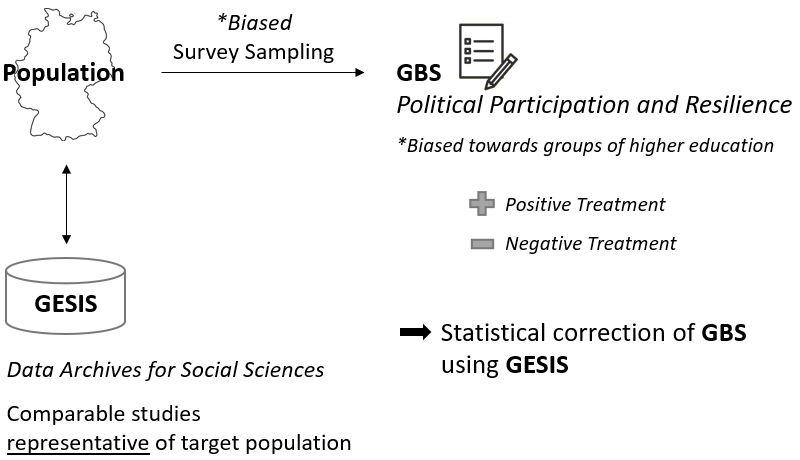
\includegraphics[scale=0.64,angle=0]{fig/overview}
		\label{project}
		\caption{Auxiliary information GESIS linked to GBS so that expected bias can be detected and corrected for. In addition, GBS contains an attribute for positive or negative treatment of survey participants for further analysis.}
	\end{center}
\end{figure}

Depending on the definition of MRS, there are two possible ways to tackle this problem:

\begin{enumerate}

\item Search algorithm with objective scoring function.

\item Try to avoid giving the synthesized data properties that makes it possible for a learning algorithm to distinguish synthesized from non-synthesized example such as if all the synthesized data comes from one of 20 car designs, or all the synthesized audio comes from only 1 hour of car noise. This advice can be hard to follow. 

\end{enumerate}

\section{Machine Learning for Complex Survey Data}

9.   Incorporate complex survey data features 

%http://ccsg.isr.umich.edu/index.php/chapters/statistical-analysis-chapter#nine

Several approaches exist to deal with positive and unlabeled data. The most straightforward one is to assume that all the unlabeled data are negative and simply apply standard machine learning techniques (Neelakantan, Roth, and McCallum 2015). A second approach is to select some of the unlabeled examples that are very different from the positively labeled ones and label them as negative. A classifier is then learned using the given positive examples and inferred negative examples (Liu et al. 2002; Li and Liu 2003; Yu, Han, and Chang 2004; Yu 2005; Li et al. 2009; Nguyen, Li, and Ng 2011). A third approach is to employ an evaluation metric that only uses positive, or positive and unlabeled data (Muggleton 1996; Lee and Liu 2003; Claesen et al. 2015a). Using this metric, one can tune for the best class weights or regularization settings (Lee and Liu 2003; Liu et al. 2005; Mordelet and Vert 2014; Claesen et al. 2015c). A final approach is to explicitly consider the class prior. It can be used to either adapt algorithms to incorporate this information during learning (Denis 1998; Liu et al. 2003; Zhang and Lee 2005; Denis, Gilleron, and Letouzey 2005; Elkan and Noto 2008) or as a preprocessing step to assign weights to the unlabeled examples (Elkan and Noto 2008). Because the class prior is often not known, several methods were proposed in the last decade to estimate it from the positive and unlabeled data (Elkan and Noto 2008; du Plessis and Sugiyama 2014; du Plessis, Niu, and Sugiyama 2015; Jain, White, and Radivojac 2016; Jain et al. 2016; Ramaswamy, Scott, and Tewari 2016) 

Both theoretical and practical results show that the out-of sample error increases proportionally to the distribution shift [2, 20]. To compensate for the degradation in performance, many techniques have been designed to reduce the effects of covariate shift.
% [1,4,9,10,12,15,16,17,18,19,21].	

\section{Outline}

I will frequently refer to decision tree theory. You will need a basic understanding of what they are to follow this text. Decision trees have performaned slightly outperformed comparable discriminative.

The remainder of this thesis is organized as follows. Section 2 starts with an initial data analysis step and focuses more narrowly on checking assumptions required for model fitting and hypothesis testing, i.e. handling missing values and making transformations of variables. Section 3 discusses the feasibility of learning in a binary classification setting. To estimate model performance in the absence of labeled negatives, standard evaluation metrics are adapted using an initial ranking model. Discriminative ensemble models are trained on positive and unlabaled data in Section 4 to label instances as representative that cannot be distinguished from the out-of-sample distribution. The resulting maximal representative subset of GBS is presented in Section 5 and compared to GBS and GESIS regarding political participation and resilience. Related work is discussed in Section 6 and Section 7 concludes.
